\documentclass[letterpaper]{article}
\usepackage[preprint]{aaai2027} % TRIAL: author-identifiable, suppresses AAAI copyright for Springer-workshop preview; seek organizer confirmation
\usepackage[hyphens]{url}
\usepackage{graphicx}
\urlstyle{rm}
\def\UrlFont{\rm}
\usepackage{natbib}
\usepackage{caption}
\frenchspacing
\usepackage{booktabs}
\usepackage{amsmath,amssymb}
\pdfinfo{/TemplateVersion (2027.2)}
\setcounter{secnumdepth}{2}
\title{Separating Threshold Failure from Information Limits in Repeated LLM Inference}
\author{Takeshi Hara\textsuperscript{\rm 1}, Hideya Konishi\textsuperscript{\rm 2}}
\affiliations{
\textsuperscript{\rm 1}Department of Diagnostic and Interventional Radiology, St. Marianna University School of Medicine, Kawasaki, Japan\\
\textsuperscript{\rm 2}Department of Radiation Oncology, St. Marianna University School of Medicine, Kawasaki, Japan\\
takeshi.hara@marianna-u.ac.jp
}
\usepackage{placeins}
\begin{document}
\maketitle



\begin{abstract}
Failure of one rule to meet a risk--coverage target does not establish infeasibility for all selectors using that observation representation. For fixed labeled data, an optimistic relaxation enforces equal acceptance probabilities only within verified observation-equivalence blocks, allowing correctness-based separation elsewhere to bound coverage. For prespecified disjoint candidate blocks with known sizes and error counts, we determine the minimum certifying block count and verify bounds using exact rational arithmetic.

We audited 174 patient--model records (90 pancreatic CT patients; 20 diagnoses each). At 5\% risk, one verified PDAC$\times$20 block (32 records, six errors) excluded 50\% coverage in all-category GPT ($n=86$; bound 45.98\%); 45\% required two blocks (44.40\%). In PDAC/NET GPT ($n=75$), a post-hoc deterministic rule using stored entropy and modal diagnosis accepted 43 records (two errors; 57.33\% coverage, 4.65\% risk). In 400 synthetic datasets at 5\% risk, 2,167 case-wise-feasible but information-infeasible dataset--target pairs required a median of three blocks; 22.1\% required one. Across 200 paired seeds, correctness-independent 16-ary noise raised mean training-oracle coverage by 5.29 percentage points; test-risk difference at 50\% coverage was +0.005 percentage points (95\% bootstrap CI, $-0.044$ to $+0.056$).

Verified input equalities can certify fixed-sample, representation-restricted infeasibility without reconstructing all equivalence classes; in-sample oracle gains cannot establish independent-test improvement.
\end{abstract}

\section{Introduction}

In repeated-output clinical LLM selective prediction, failure of a monotone entropy threshold to meet a risk--coverage target may reflect an inadequate selection rule, mixed correctness among records identical under the permitted observations, or insufficient correct fixed predictions even with case-wise identification. These constraints can coexist; threshold failure alone does not establish which one limits achievable coverage.

We audit empirical risk--coverage feasibility on fixed predictions under a specified observation representation, such as repeated diagnostic labels and the recorded majority diagnosis. Selectors must assign identical acceptance probabilities to identical observations. We ask whether a target can be certified as infeasible even for a post-hoc oracle designed with full knowledge of correctness and allowing outcome-independent randomization.

For fixed predictions on a labeled cohort, verified input equalities can rule out a cohort-wide risk--coverage target for every selector restricted to the specified representation. We verify exclusion bounds in exact rational arithmetic. An explicit rule establishes in-sample feasibility. The target remains unresolved when neither form of evidence is available.

Given disjoint candidate equality blocks, we compute the minimum number needed for that exclusion. At 5\% selective risk, one verified block excluded 50\% coverage for all-category GPT, whereas 45\% coverage required two. We measure how the minimum changes when errors concentrate in one block or disperse across several.

We also test what a rise in empirical oracle coverage implies. A rule using stored entropy and the majority diagnosis demonstrates feasibility on the PDAC/NET subset. Random-symbol and outcome-correlated controls compare gains from splitting training records with changes in selective risk on independent synthetic test sets.

\section{Related Work}

\subsection{Optimal Selection and Empirical Auditing}

\citet{franc2023} characterized optimal randomized selection for reject-option classification. \citet{kuboyama2026} studied the number of reference labels needed to certify model choice among fixed candidates under AUGRC. In contrast, we assume known correctness and count verified input-equality blocks sufficient to exclude an empirical risk--coverage target.

\subsection{Oracle Gaps and Observation Equivalence}

\citet{rabanser2025} analyzed the gap between selective classifiers and a perfect-ordering oracle. \citet{kim2026} showed that answer distributions alone cannot always distinguish correct from incorrect majority answers. Here, selectors must assign equal acceptance probabilities to identical recorded diagnostic-label representations. We determine when partial knowledge of these equalities suffices to exclude a whole-cohort target.

\subsection{Black-Box Uncertainty and Entropy-Based Abstention}

\citet{lin2024} studied uncertainty measures from black-box LLM generations, while \citet{phillips2026} reported model-dependent limitations of entropy-based selective prediction and evaluated supervised correctness probes. We instead audit fixed diagnostic-label information through four nested selector classes: monotone thresholds on stored label entropy, arbitrary entropy-based rules, rules additionally using the recorded modal diagnosis, and rules using the full diagnostic-label sequence together with that diagnosis. This hierarchy distinguishes threshold failure from information-restricted infeasibility.

\subsection{Statistical Risk Guarantees and Fixed-Sample Reachability}

\citet{geifman2017} and \citet{angelopoulos2025} developed high-probability population-risk control for calibrated prediction or selection policies. We instead audit empirical risk--coverage reachability on a fixed dataset under specified observation constraints. Verified input-equality constraints can certify that no restricted selector meets a target, while correctness-informed witnesses establish in-sample feasibility. Neither result guarantees prospective risk control.

\section{Problem Formulation and Audit Certificates}

\subsection{Fixed Predictions, Observations, and Empirical Risk}

For each evaluated model, let the audited dataset be \(D = \left\{ \left( S_{i},{\widehat{y}}_{i},y_{i} \right) \right\}_{i = 1}^{n}\), where \(S_{i} = \left( z_{i,1},\ldots,z_{i,T} \right)\) is the ordered sequence of \(T = 20\) recorded diagnostic category labels, \({\widehat{y}}_{i}\) is the recorded majority diagnosis, and \(y_{i}\) is the reference ground-truth (GT) category. Let \(\ell_{i} = \mathbf{1}\left\{ {\widehat{y}}_{i} \neq y_{i} \right\} \in \left\{ 0,1 \right\}\) denote the fixed prediction error indicator. The selector cannot alter \({\widehat{y}}_{i}\). The label sequence \(S_{i}\) contains only categorical diagnostic labels and excludes free-text rationales, self-reported confidence, clinical imaging features, and patient identifiers.

We define the sequence-level label representation as \(Z_{S,i} = \left( S_{i},{\widehat{y}}_{i} \right)\). Including \({\widehat{y}}_{i}\) explicitly preserves the hierarchy of policy classes without fabricating post-hoc tie-breaking rules for the minority of records (7/174) where \(S_{i}\) exhibits a tied mode. Whenever \({\widehat{y}}_{i}\) is uniquely determined by \(S_{i}\), \(Z_{S,i}\) is informationally equivalent to \(S_{i}\).

A selector restricted to an observation representation \(Z\) assigns an acceptance probability \(q_{i} = g\left( Z_{i} \right) \in \lbrack 0,1\rbrack\) to record \(i\). Crucially, \(g\) must assign identical probabilities to identical observations (\(Z_{i} = Z_{i'} \Longrightarrow q_{i} = q_{i'}\)), and any execution-time randomization is independent of \(\ell_{i}\). Although an oracle selector may inspect all ground-truth labels \(\ell_{i}\) during rule design, it cannot split records within an equivalence class of \(Z\). Empirical coverage and selective risk on \(D\) are defined as:

\[\begin{aligned}
C_D(g) &= \frac{1}{n}\sum_{i=1}^n q_i,\\
R_D(g) &= \frac{\sum_{i=1}^n \ell_i q_i}{\sum_{i=1}^n q_i}
\quad (C_D(g)>0).
\end{aligned}\]

\subsection{Policy Classes and Information Hierarchy}

Let \({\widetilde{H}}_{i}\) denote the recorded normalized Shannon entropy computed over the three diagnostic categories (PDAC, NET, Other) and stored to three decimal places. Even when evaluating the PDAC/NET GT subset, \({\widehat{y}}_{i}\), \({\widetilde{H}}_{i}\), and the three-category output space remain unchanged. We compare four nested policy classes: (i) monotone low-entropy thresholds \(g_{t}\left( \widetilde{H} \right) = \mathbf{1}\left\{ \widetilde{H} \leq t \right\}\), (ii) arbitrary randomized policies \(g\left( \widetilde{H} \right)\), (iii) class-conditional entropy policies \(g\left( \widetilde{H},\widehat{y} \right)\), and (iv) full-sequence policies \(g\left( Z_{S} \right)\). Denoting the exact in-sample oracle optimum for representation \(Z\) at risk budget \(\alpha\) as \(C_{Z}^{\text{opt}}(\alpha)\), informational inclusion implies:

\[C_{\text{low-}H}^{\text{opt}}(\alpha) \leq C_{\widetilde{H}}^{\text{opt}}(\alpha) \leq C_{\left( \widetilde{H},\widehat{y} \right)}^{\text{opt}}(\alpha) \leq C_{Z_{S}}^{\text{opt}}(\alpha).\]

These inequalities hold in-sample when summaries are consistently derived from \(Z_{S}\), but imply neither strict inequality at every \(\alpha\) nor out-of-sample generalization.

\subsection{Equivalence Constraints and the Optimistic Relaxation}

Partition the \(n\) records into equivalence blocks \(j \in \left\{ 1,\ldots,M \right\}\) sharing identical values of \(Z\), with block size \(n_{j}\), error count \(e_{j} = \sum_{i \in B_{j}}^{}\ell_{i}\), and shared acceptance probability \(q_{j} \in \lbrack 0,1\rbrack\). When all blocks of \(Z\) are known, \(C_{Z}^{\text{opt}}(\alpha)\) is given by the linear program (LP):

\[\begin{aligned}
C_Z^{\mathrm{opt}}(\alpha) &= \max_{q\in[0,1]^M}\frac{1}{n}\sum_{j=1}^M n_jq_j,\\
\mathrm{subject\ to}\quad &\sum_{j=1}^M(e_j-\alpha n_j)q_j\leq0.
\end{aligned}\]

Even when full sequences are only partially reconstructed or audited, specific observational collisions---such as unanimous sequences (\(\text{PDAC} \times 20\) or \(\text{NET} \times 20\))---can be verified. Retaining only a verified subset of equality constraints while permitting unconstrained case-wise error separation on all remaining records defines an optimistic relaxation with optimum \(U_{\text{coll}}(\alpha)\).

\textbf{Proposition 1 (Upper bound from partial equivalence constraints).} If every retained equality constraint groups records with truly identical representations \(Z_{S}\), then \(C_{Z_{S}}^{\text{opt}}(\alpha) \leq U_{\text{coll}}(\alpha)\).

\emph{Proof sketch.} Any policy \(g\left( Z_{S} \right)\) respects all true equality constraints of \(Z_{S}\). Dropping unverified equality constraints expands the feasible set of the LP, which cannot decrease the maximum achievable coverage. Conversely, merging records based solely on coarse scalar summaries (e.g., equal \(\widetilde{H}\) despite distinct \(S\)) imposes artificial constraints and need not bound \(C_{Z_{S}}^{\text{opt}}(\alpha)\). Adding further verified equality constraints monotonically tightens \(U_{\text{coll}}(\alpha)\). \(\square\)

\subsection{Rational Certificates and Minimum Certifying Block Counts}

By Lagrangian duality, for any multiplier \(\lambda \geq 0\), every feasible solution \(q\) of the relaxed LP satisfies:

\[\begin{aligned}
C_D(q) &= \frac{1}{n}\sum_j n_jq_j \\
&\leq\frac{1}{n}\sum_j [n_j-\lambda(e_j-\alpha n_j)]q_j \\
&\leq\frac{1}{n}\sum_j\max\{0,n_j-\lambda(e_j-\alpha n_j)\}\\
&\equiv U(\lambda;\alpha).
\end{aligned}\]

If \(U(\lambda;\alpha) < c\) for some \(\lambda \geq 0\), the requirement \(\left( R_{D} \leq \alpha,\, C_{D} \geq c \right)\) is certified as infeasible. While any \(\lambda \geq 0\) yields a valid upper bound, exhibiting a primal feasible vector \(q\) and a rational multiplier \(\lambda \geq 0\) such that \(C_{D}(q) = U(\lambda;\alpha)\) in exact rational arithmetic certifies exact optimality without relying on floating-point solver tolerances.

\paragraph{Minimum Certifying Block Counts.}
Consider \(m\) prespecified, pairwise-disjoint candidate equality blocks, each verified to contain identical observations under the specified representation, with known sizes \(n_j\) and error counts \(e_j\). The fixed cohort contains \(n\) records and \(E\) errors, with correctness labels assumed known. Let \(0\leq\alpha<1\) and \([x]_{\mathrm{pos}}=\max\{x,0\}\). With no retained equality constraints, the case-wise dual upper bound, expressed in expected accepted records, is
\[
B_0(\lambda)
=(n-E)(1+\alpha\lambda)
+E[1-(1-\alpha)\lambda]_{\mathrm{pos}},
\qquad \lambda\geq 0.
\]

Enforcing equality within candidate block \(j\) reduces this expression at a fixed \(\lambda\) by
\[
\begin{aligned}
\Delta_j(\lambda)
={}&(n_j-e_j)(1+\alpha\lambda)\\
&+e_j[1-(1-\alpha)\lambda]_{\mathrm{pos}}\\
&-[n_j-\lambda(e_j-\alpha n_j)]_{\mathrm{pos}}
\geq 0.
\end{aligned}
\]
Because candidate blocks are disjoint, these reductions are additive at the same \(\lambda\). Thus, selecting the \(k\) largest reductions minimizes the dual expression among subsets of at most \(k\) blocks at that multiplier. Reductions optimized separately at different multipliers are not additive.

For any subset \(J\), the dual expression is
\(B_0(\lambda)-\sum_{j\in J}\Delta_j(\lambda)\).
Subset selection and minimization over \(\lambda\) may be interchanged because both are minimizations. Each fixed-subset dual is piecewise linear, with an optimum attained at a point in the finite set
\[
\Lambda=
\left\{0,\frac{1}{1-\alpha}\right\}
\cup
\left\{
\frac{n_j}{e_j-\alpha n_j}:
e_j>\alpha n_j
\right\}.
\]
Writing \(\Delta_{(r)}(\lambda)\) for the \(r\)th largest reduction at \(\lambda\), the exact smallest optimistic coverage upper bound obtainable from at most \(k\) blocks is
\[
V_k(\alpha)=
\frac{1}{n}\min_{\lambda\in\Lambda}
\left[
B_0(\lambda)-
\sum_{r=1}^{k}\Delta_{(r)}(\lambda)
\right].
\]

For a coverage target \(0<c\leq1\), the minimum certifying block count relative to the candidate family is the smallest \(k\in\{0,\ldots,m\}\) satisfying \(V_k(\alpha)<c\). Equality with \(c\) does not certify exclusion. If no such \(k\) exists, the candidate blocks do not certify infeasibility. The procedure examines at most \(m+2\) candidate multipliers without enumerating all \(2^m\) block subsets. This count measures verified equality blocks, not the costs of discovering them, obtaining correctness labels, or verifying their equality.

\subsection{Tri-State Audit Outcomes, Fixed-Coverage Risk, and Case-Wise Gap}

For a target pair ($\alpha$, c), the audit distinguishes three evidence-dependent outcomes: (1) \textbf{In-sample feasible}, when an explicit selection rule restricted to the specified observation representation satisfies both the empirical risk and coverage requirements; (2) \textbf{Infeasible under the specified representation}, when a verified upper bound falls strictly below c; and (3) \textbf{Unresolved}, when neither a feasibility witness nor an excluding bound has been established. Unresolved denotes insufficient evidence for either conclusion, not a third state of mathematical feasibility. A valid witness provides a lower bound, and a partial-equivalence relaxation provides an upper bound, on the optimal in-sample coverage attainable under the specified representation.

Equivalently, at a positive target coverage c, we minimize expected empirical selective risk subject to the verified equality constraints and expected coverage exactly c. If this relaxed minimum exceeds $\alpha$, every restricted selector attaining coverage at least c is excluded, because uniform scaling of acceptance probabilities preserves expected selective risk. Let A denote the empirical accuracy of the fixed diagnoses. For 0 $\leq$ $\alpha$ $<$ 1, a case-wise oracle with knowledge of individual correctness, but without altering predictions, attains maximum coverage min\{1, A/(1$-$$\alpha$)\}. The difference between this case-wise optimum and the partial-equivalence upper bound therefore provides a lower bound on the empirical coverage loss attributable to observational indistinguishability under the specified representation. These results are conditional on the audited cohort and do not provide prospective risk guarantees.

\subsection{Partial Evidence, Representation Refinement, and Provenance Controls}

To evaluate how partial collision evidence tightens coverage upper bounds, we audited all eight (2$^{3}$) subsets of the three multi-record sequence blocks in the clinical data. In a first synthetic benchmark, we evaluated 400 datasets (n = 100 or 500; 50 seeds per sample size and error structure) across four structures: outcome-homogeneous blocks, errors concentrated in unanimous blocks, errors dispersed across non-unanimous blocks, and high-uniqueness sequences, with a baseline error rate of 30\%. Across risk budgets from 0\% to 20\% in 1-percentage-point increments and coverage targets from 10\% to 90\% in 5-percentage-point increments, we assessed bound slack and the proportion of information-infeasible requirements excluded as 0\%, 25\%, 50\%, 75\%, or 100\% of collision blocks were disclosed in random or descending-size order. Information-infeasible requirements were defined as those feasible for the case-wise oracle but infeasible under the full observation representation.

In a separate minimum-evidence benchmark, we generated 400 additional synthetic datasets, each comprising 120 records and 36 errors (100 datasets per block structure). We evaluated three risk budgets (2\%, 5\%, and 10\%) and 17 coverage targets ranging from 40\% to 80\% in 2.5-percentage-point increments. The minimum certifying block count was computed using the dual-based procedure in Section 3.4 and independently verified by exhaustive enumeration of all subsets of at most seven pairwise disjoint candidate blocks. We compared this minimum with descending-block-size and random verification orders. Multiple targets evaluated on the same dataset shared records and were not treated as independent datasets. All minimum-certificate analyses were retrospective and assumed known correctness labels.

For the clinical representation control, we appended independently generated k-ary random symbols (k = 2, 4, or 16) to the archived 20-output label sequence and recorded majority diagnosis. Symbols were generated without using correctness labels, separately for each cardinality and evaluation condition. We performed 200 random assignments per cardinality and condition, yielding 2,400 optimizations at $\alpha$ = 0.05. For each assignment, we calculated the maximum in-sample coverage and checked the optimum using exact-rational primal--dual certificates. The rerun used equality-block sizes and error counts reconstructed from archived clinical audit summaries, without rereading the original patient-level files or modifying diagnoses, ground-truth mappings, or cohort definitions. Because the earlier 50-seed random-number stream was unavailable, these were new 200-seed Monte Carlo experiments rather than reproductions of the original assignments.

Separately, we conducted a paired 200-seed synthetic negative/positive-control benchmark. Each seed generated independent training (n = 500), calibration (n = 500), and test (n = 5,000) samples. The binary base feature X followed $\Pr(X=0)=0.4$, with $\Pr(\mathrm{error}\mid X=0)=0.01$ and $\Pr(\mathrm{error}\mid X=1)=0.35$. At $\alpha$ = 0.05, its population-optimal coverage was 45.33\%. We added either uniform 2-, 4-, or 16-ary nuisance symbols generated conditionally independently of correctness, or artificial binary signals matching the error indicator with probabilities of 0.90 or 0.98. These positive-control signals were generated using correctness by design and were not intended as deployable clinical features.

For each representation, we first computed a correctness-informed in-sample oracle on the training sample. Separately, we fitted smoothed error scores using training labels, selected a randomized threshold on the calibration sample to maximize empirical coverage subject to a 5\% empirical risk constraint, and evaluated the resulting fixed rule on an independent test sample.

As a distinct diagnostic analysis, we compared test selective risk at exactly 50\% coverage, randomizing within tied scores. The test feature distribution was used to determine the coverage-matched threshold, but test correctness labels were not used to fit the scores. This comparison was not the calibration-selected operating point and did not establish a prospective 5\% risk guarantee. We reported paired differences across seeds with 95\% bootstrap intervals and performed sensitivity analyses at $\alpha$ = 0.02 and 0.10.

Using archived raw outputs, we reconstructed 52 diagnostic sequences (1,040 labels) that had been unavailable in the initial sequence-level audit. We verified agreement between recomputed entropies and stored three-decimal values across all 174 patient--model records (3,480 diagnostic labels). Runs were ordered by their archived run indices, and the recorded majority diagnoses were preserved in all seven records with tied modal categories rather than being reassigned post hoc. For GPT case005, which had 21 candidate outputs, the prespecified rule retaining the first 20 valid runs and the archived audit logs confirmed inclusion of Run01--20 and exclusion of Run21.

Archived clinical outputs were collected through the ChatGPT (“GPT 5.2 Instant”; May 4–21, 2026) and Gemini (“Gemini3 Fast mode”; May 9–16, 2026) web interfaces without API access. Each run used the fixed version-4 prompt, identical images in the same order, and a fresh chat session. The prompt was finalized before E2 cohort evaluation. Nominal temperature (0.3) and top-p (1.0) were specified in the prompt, but backend model versions and decoding settings could not be verified.

\section{Results}

\subsection{Clinical Evaluation and Distinct Audit Outcomes}

We audited 174 patient--model records from 90 pancreatic CT patients (86 GPT and 88 Gemini records; 20 inferences per record). Evaluations were performed separately by model. The PDAC/NET subsets were defined by ground truth solely for retrospective stratification, not as deployable selection criteria. The illustrative audit specification was selective risk $\leq$5\% with coverage $\geq$50\%.

No nonempty selection obtained by a monotone low-entropy threshold satisfied the 5\% empirical selective-risk constraint in any of the four evaluations (Table~\ref{tab:1}). Nevertheless, the attainable coverage and audit conclusions differed across information classes.

\begin{table*}[t]
\centering
\small
\setlength{\tabcolsep}{3.7pt}
\begin{tabular}{llrrrrrrr}
\toprule
Evaluation set & Model & $n$ & Low-$H$ & $g(\widetilde H)$ & $g(\widetilde H,\hat y)$ & $g(Z_S)$ & $U_{\rm coll}$ & Case-wise\\
\midrule
All GT categories & GPT & 86 & 0.00 & 9.97 & 17.44 & 44.40 & 44.40 & 67.32\\
All GT categories & Gemini & 88 & 0.00 & 4.26 & 18.81 & 36.05 & 36.05 & 45.45\\
PDAC/NET subset & GPT & 75 & 0.00 & 26.67 & 58.67 & 77.04 & 77.04 & 77.19\\
PDAC/NET subset & Gemini & 77 & 0.00 & 11.99 & 34.03 & 39.41 & 39.41 & 50.58\\
\bottomrule
\end{tabular}
\caption{Maximum in-sample coverage (\%) at 5\% selective risk for nested selector classes and oracles. Low-$H$ coverage 0.00\% indicates that no nonempty threshold selection met the risk constraint; risk at zero coverage is undefined. Optima permit randomized acceptance unless stated otherwise.}
\label{tab:1}
\end{table*}

In all-category GPT, the full-sequence oracle reached at most 44.40\% coverage at 5\% risk, compared with 67.32\% under case-wise error identification; the minimum sequence-restricted risk at 50\% coverage was 6.54\%. In all-category Gemini, even the case-wise oracle reached only 45.45\%, so fixed-prediction correctness alone excluded the target. Conversely, in PDAC/NET GPT, a deterministic post-hoc rule using recorded entropy and modal diagnosis accepted 43/75 records with two errors (57.33\% coverage; 4.65\% risk), establishing in-sample feasibility. PDAC/NET Gemini remained infeasible under the full-sequence representation (39.41\% coverage versus 50.58\% case-wise; Table~\ref{tab:1}). These findings concern fixed predictions and retrospective evaluation strata, not deployable clinical selection rules.


\begin{figure*}[t]
\centering
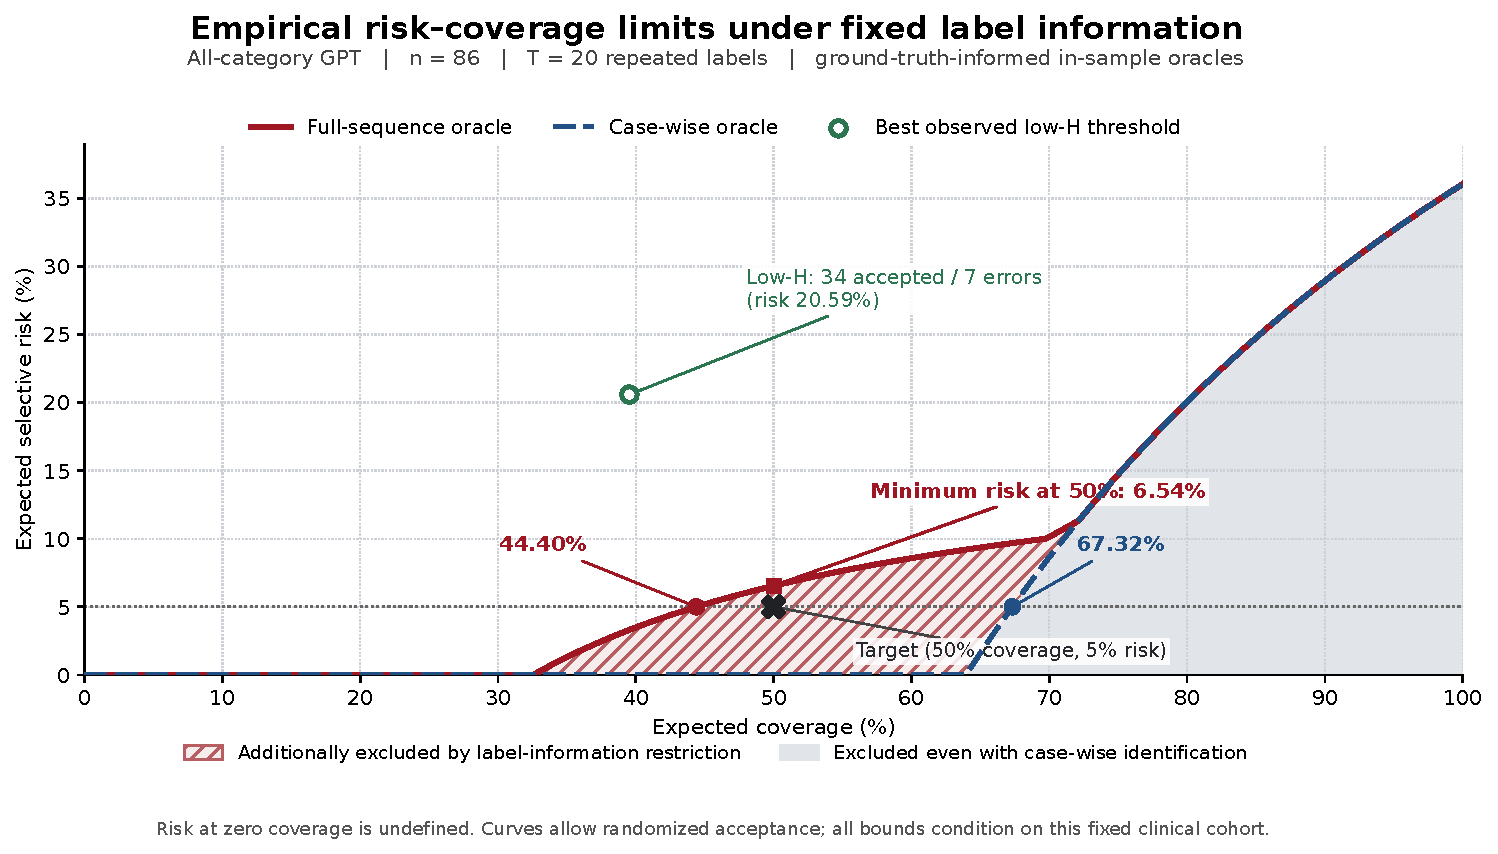
\includegraphics[width=0.95\textwidth]{figure1.pdf}
\caption{Empirical risk--coverage frontiers for all-category GPT (n = 86). The red curve shows the minimum selective risk under the recorded diagnostic-label sequence and modal diagnosis; the blue curve represents the case-wise oracle with individual error identification. Both are post-hoc and allow randomized acceptance without changing predictions. Red hatching indicates targets additionally excluded by the sequence restriction; gray shading indicates targets excluded even case-wise. At 5\% risk, maximum coverage was 44.40\% and 67.32\%, respectively. The cross marks the 50\%-coverage/5\%-risk target, excluded under the sequence restriction (minimum risk at 50\% coverage: 6.54\%). The green point denotes the best observed nonempty low-entropy threshold. These are fixed-sample results, not prospective risk guarantees.}
\label{fig:1}
\end{figure*}


\subsection{Minimum Evidence Needed to Exclude a Target}

The all-category GPT evaluation comprised \(n=86\) patient--model records, including \(E=31\) errors. Three unanimous-sequence blocks contained multiple records: PDAC$\times$20 (\(n_D=32,e_D=6\)), NET$\times$20 (\(n_N=2,e_N=1\)), and Other$\times$20 (\(n_O=2,e_O=0\)). The remaining 50 non-unanimous records comprised 26 correct and 24 erroneous predictions.

At a 5\% risk budget (\(\alpha=1/20\)), retaining \textbf{only} the PDAC$\times$20 equality leaves 54 records (29 correct and 25 erroneous) optimistically distinguishable. The rational dual multiplier \(\lambda=80/11\) gives the following coverage upper bound:

\[
U_{\{D\}}(1/20)=\frac{435}{946}=45.98\%<50\%.
\]

This bound is attained in the relaxed LP by accepting all 29 correct records outside the block, assigning an acceptance probability of \(q_D=29/88\) to the PDAC$\times$20 block, and rejecting all remaining records. Without any equality constraints, the case-wise upper bound is \(U_{\varnothing}(1/20)=550/817>50\%\). Thus, \textbf{one verified block is both necessary and sufficient to exclude 50\% coverage}, relative to the candidate blocks.

Retaining \textbf{both} PDAC$\times$20 and NET$\times$20 equalities leaves 52 records outside these blocks: 28 correct (including both Other$\times$20 records) and 24 erroneous. At the same dual multiplier \(\lambda=80/11\), the coverage upper bound is:

\[
U_{\{D,N\}}(1/20)=\frac{210}{473}=44.40\%<45\%.
\]

A matching feasible solution of the relaxed primal LP assigns acceptance probabilities of \(q_D=7/22\) and \(q_N=0\) to the PDAC$\times$20 and NET$\times$20 blocks, respectively, accepts all 28 correct outside records, and rejects all 24 outside errors. The expected accepted and error counts are \(420/11\) and \(21/11\), giving exactly 5\% risk and \(210/473\) (44.40\%) coverage. Since the tightest one-block bound, \(435/946\), exceeds 45\%, whereas the two-block bound, \(210/473\), falls below 45\%, \textbf{two verified blocks are necessary and sufficient to exclude the 45\% target within the prespecified candidate family}.

In the PDAC/NET Gemini evaluation, the NET$\times$20 block of 13 records alone excluded 50\% coverage, with an optimistic upper bound of 44.38\% (Table~\ref{tab:2}).

\begin{table*}[t]
\centering
\small
\setlength{\tabcolsep}{5pt}
\begin{tabular}{lrrrr}
\toprule
Evaluation condition & No blocks & PDAC$\times$20 & NET$\times$20 & Both blocks \\
\midrule
All-category GPT ($n=86$) & 67.32 & \textbf{45.98} & 67.32 & \textbf{44.40}\\
All-category Gemini ($n=88$) & \textbf{45.45} & 45.45 & 39.85 & 36.05\\
PDAC/NET GPT ($n=75$) & 77.19 & 77.19 & 77.19 & 77.04\\
PDAC/NET Gemini ($n=77$) & 50.58 & 50.16 & \textbf{44.38} & \textbf{39.41}\\
\bottomrule
\end{tabular}
\caption{Optimistic coverage upper bounds (\%) at 5\% risk from verified equality blocks. No blocks gives the case-wise oracle. Both verified blocks attained the full-sequence oracle optimum in these evaluations. All bounds permit randomized acceptance on the fixed labeled cohort.}
\label{tab:2}
\end{table*}

In the first 400-dataset structural benchmark, unanimity-only evidence was tight when mixed-outcome collisions were concentrated in unanimous blocks. When such collisions were dispersed across non-unanimous blocks, however, unanimity-only bounds excluded only 5.72\% (n = 100) and 5.24\% (n = 500) of information-infeasible targets.

In a separate 400-dataset benchmark, dual sorting and exhaustive enumeration agreed on the minimum certificate count across all 20,400 dataset--risk--coverage evaluations. At 5\% risk, 2,167 of 6,800 dataset--target pairs were case-wise feasible but information-infeasible. Among these, the median minimum certificate comprised three blocks (median 38 records), and 479/2,167 (22.1\%) required only one block. One-block certificates occurred for 47.3\% of concentrated-error targets but none of the dispersed-error targets. Multiple targets evaluated on the same dataset were not independent.

\subsection{In-Sample Oracle Inflation after Representation Refinement}

Appending random symbols generated independently of correctness increased post-hoc in-sample oracle coverage without changing the fixed diagnoses or reference labels. In all-category GPT, mean coverage rose from 44.40\% to 51.01\%, 56.44\%, and 64.71\% after adding independent 2-, 4-, and 16-ary symbols, respectively (200 assignments per cardinality). Unique record identifiers yielded the case-wise oracle ceiling of 67.32\% by construction; none of these results demonstrates held-out clinical utility.

\subsection{Independent-Test Controls for Apparent Oracle Gains}

Across 200 paired synthetic replicates, adding a correctness-independent 16-ary symbol increased mean training-set oracle coverage from 45.41\% to 50.70\%, although the population-optimal coverage remained 45.33\% for both representations at 5\% risk. Artificial signals generated with 90\% and 98\% agreement with the error indicator yielded training oracle coverages of 78.97\% and 82.21\%, respectively (Figure~\ref{fig:2}).

At calibration-selected operating points, mean test coverage/risk was 45.47\%/5.06\% for the base representation and 45.78\%/5.22\% with 16-ary noise. In a separate comparison at fixed 50\% test coverage, the paired risk difference for 16-ary noise was +0.005 percentage points (95\% paired-seed bootstrap CI, $-$0.044 to +0.056), whereas the artificial error-related signals reduced risk by 5.88 and 7.35 percentage points. This fixed-coverage comparison used test features, but not test correctness, to determine its operating point; it neither evaluates the calibration-selected policy nor establishes a 5\% risk guarantee.


\begin{figure*}[t]
\centering
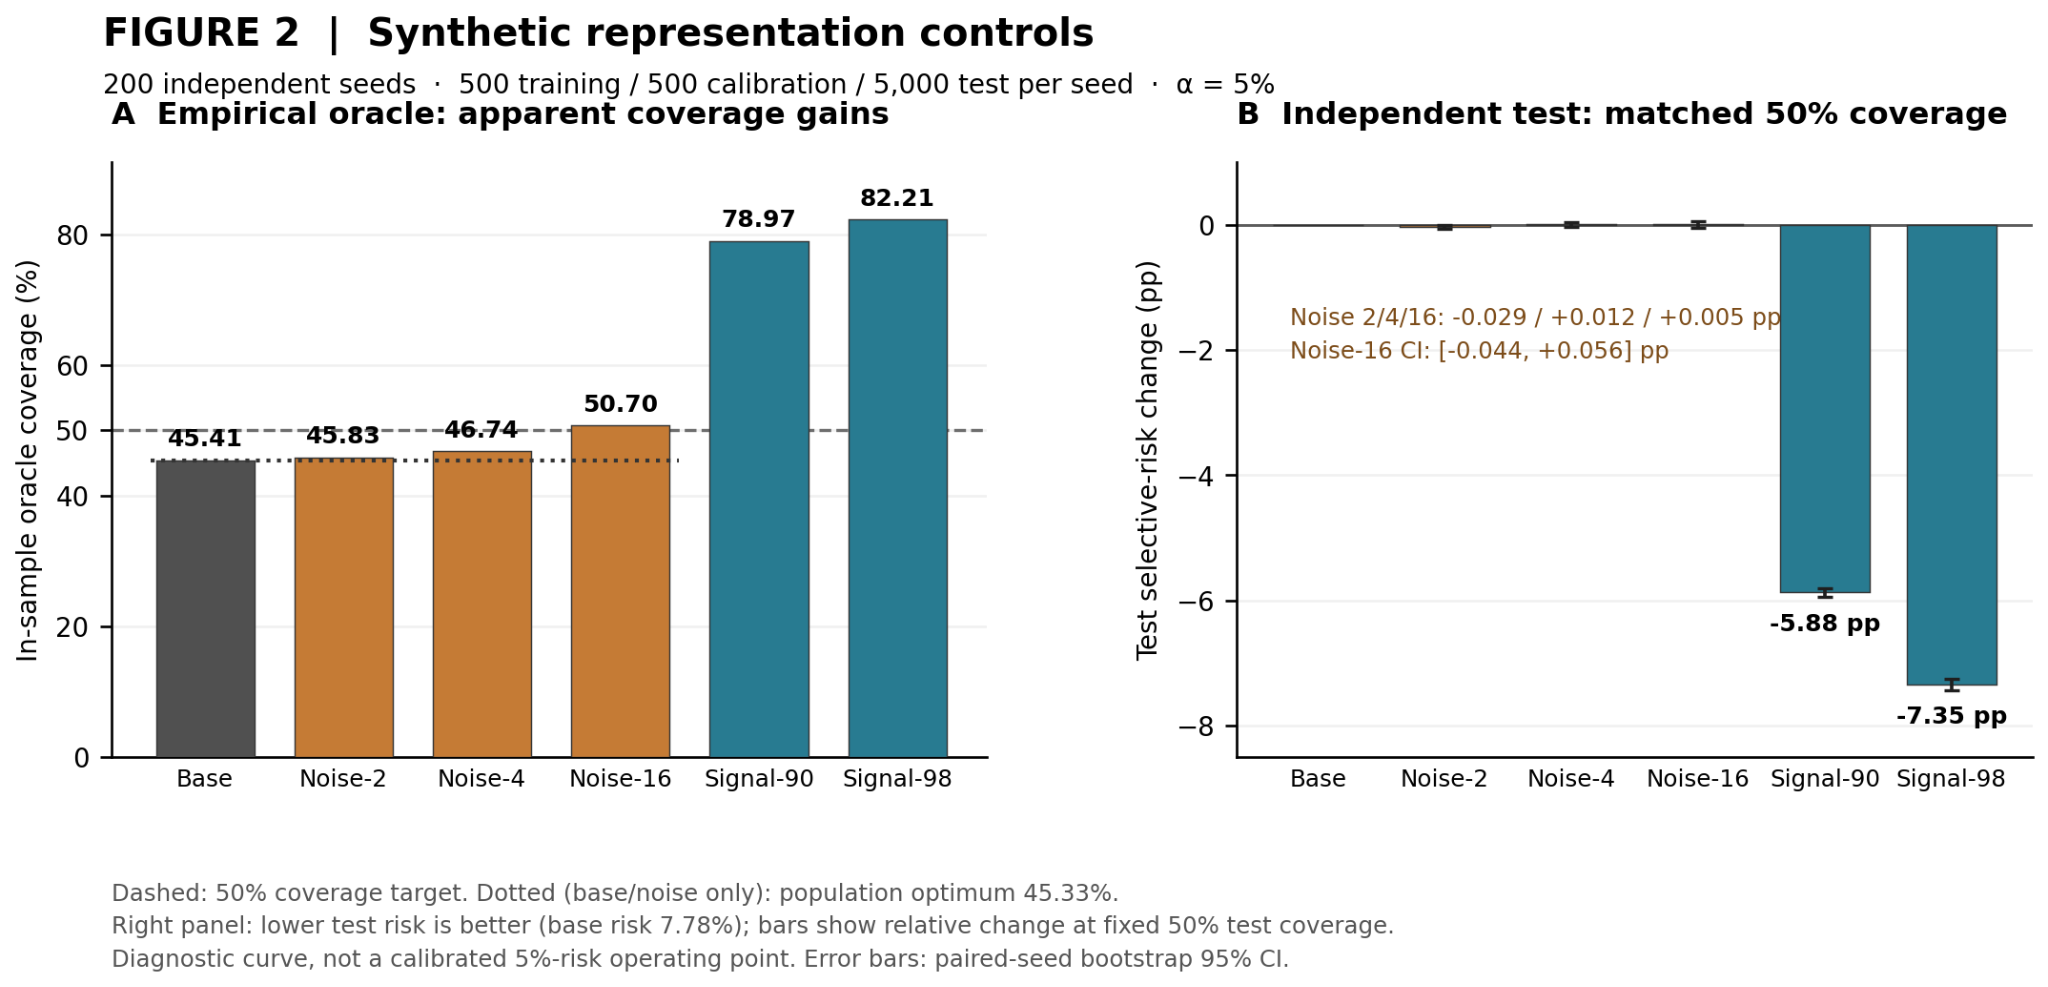
\includegraphics[width=0.95\textwidth]{figure2.png}
\caption{Synthetic representation controls across 200
paired replicates. (A) Training-set oracle coverage
after adding correctness-independent random symbols
or artificial error-related signals. (B) Paired
differences in independent-test selective risk at
fixed 50\% coverage relative to the base
representation (95\% bootstrap intervals). Negative
values indicate lower risk. The fixed-coverage
comparison does not provide prospective risk guarantees.}
\label{fig:2}
\end{figure*}


\section{Discussion}

Verified input equalities can exclude a whole-cohort risk--coverage target for every selector using a specified representation, even when most equivalence classes remain unverified. For prespecified disjoint candidate blocks with known error counts, the minimum exclusion certificate depends on both the target and the distribution of errors. An explicit witness establishes in-sample feasibility; absent either form of evidence, the verdict remains unresolved. In synthetic controls, correctness-independent representation refinements increased in-sample oracle coverage without a detected improvement in independent-test risk at matched coverage. This framework distinguishes failure of a particular threshold rule from information-restricted infeasibility.

\section{Limitations and Future Work}

Limitations. The clinical audit was retrospective and single-center (90 patients), with fixed predictions and known correctness labels. Minimum certificate counts are exact relative to prespecified disjoint candidate blocks, but do not measure the costs of discovering, verifying, or labeling those blocks. The 5\%-risk/50\%-coverage specification was illustrative, and synthetic frequencies depend on their generators. These fixed-sample results do not establish prospective clinical risk control.

Future work. Extend certificate audits to overlapping candidate blocks and measured evidence-acquisition costs, and evaluate prespecified selection policies on independent clinical cohorts under clinically defined risk--coverage targets.

\section{Conclusion}

On a fixed labeled cohort, verified input-equality blocks can exclude a whole-cohort risk--coverage target for every selector restricted to a specified representation, with the minimum certifying block count among prespecified disjoint candidates depending on the target and error structure.

\section*{Ethical Statement}

The source retrospective study was approved by the Institutional Review Board of St. Marianna University School of Medicine (No. 7224; March 12, 2026). Individual informed consent was waived, with a public opt-out procedure.

\section*{Funding and Competing Interests}

No external funding was received. The authors declare no competing interests.

\section*{Data Availability}

Patient-level imaging and clinical data are not publicly available owing to privacy and institutional restrictions.

\section*{Acknowledgments}
OpenAI's ChatGPT was used to assist with critical and structural editing of author-written drafts, focusing on clarity, logical consistency and flow, and conciseness, as well as code assistance. The authors retain full responsibility for all aspects of the study, including its design, analyses, interpretation, and final manuscript.

\bibliography{oracle_refs}

\end{document}
